\begin{figure}[!htbp]
\centering
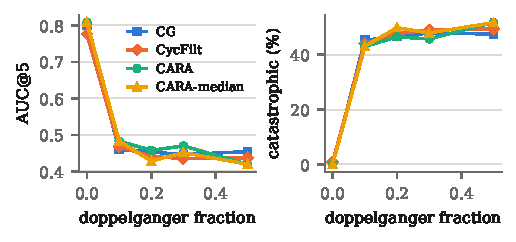
\includegraphics[width=\linewidth]{figs/dop.pdf}
\caption{Structured doppelgangers on a ring of 100 cameras around a symmetric object (5 seeds $\times$ 10 scenes per point). Spurious look-alike edges map a camera to its mirror twin and are mutually cycle-consistent. All methods fail once they are present.}
\label{fig:dop}
\end{figure}

\subsection{Structured doppelgangers}\label{sec:dop}
We place 100 cameras on a circle around an object with a $180^\circ$ symmetry and add spurious edges between cameras in the front half and cameras in the back half whose mirror twin would overlap them, with the relative rotation of the twin. These edges agree with each other around every cycle they share, so no cycle test can reject them. Without them, CARA reaches AUC@5 $0.808$ against $0.799$ for CG. With 10\% of the candidate look-alike pairs added (65 of 781 edges), every method fails: 43--45\% of cameras become catastrophic, CARA rejects only 12\% of the spurious edges, and bound coverage falls to 56\%. The picture does not change at higher fractions (\cref{fig:dop}). Neither the median triangle score nor the drift factor helps. This is the limit stated in \cref{rem:guar}: calibrated cycle tests do not replace doppelganger classifiers~\cite{cai2023doppelgangers,xiangli2025doppelgangerspp}, and the bounds are not valid when the error mechanism produces consistent wrong evidence.

